% Canonical report source. Raw LaTeX is used to preserve mathematical layout.
% Title: Expected Differences and Ranges of Correlated IQ Scores
% Audience: mathematically interested readers; prepared for Anders Hellström.
% Date: 3 September 2026. Scope: probability model, not personal assessment.

\chapter{Executive findings}
\label{ch:findings}

\begin{resultbox}[title={\textbf{The direct answer}}]
If IQ scores have common standard deviation 15, are jointly normal, and every
distinct pair has correlation 0.6, then
\[
\boxed{\E|X_1-X_2|=10.7047446969\text{ points}},\qquad
\boxed{\E(\max_{1\le j\le5}X_j-\min_{1\le j\le5}X_j)=22.0656994474\text{ points}}.
\]
The expected signed difference is zero when the two means are equal.
\end{resultbox}

These are exact expectations under a specified probability model. They are not
empirical estimates obtained from a sample of people taking real IQ tests.
The decimal values are numerical evaluations of proved formulas; reporting
10.70 and 22.07 points is normally sufficient.

The question continued from the preceding analysis is: what is the average
difference between two IQ tests when their correlation is 0.6, and what is the
average maximum-minus-minimum across five such tests? The essential task is to
identify what follows from correlation, what needs a distributional assumption,
and how simulation can check the implementation without replacing a proof.

\section{The assumptions that make the question determinate}

\begin{tblr}{colspec={Q[l,wd=42mm] X[l]},row{1}={font=\bfseries,bg=pale},
  hline{1,2,Z}={.5pt},cells={valign=t},rowsep=3pt}
Component & Assumption used for the main answer \\
Population & A randomly selected person from one defined population takes the same fixed set of tests. \\
Score scale & Every test has the same mean $\mu$ and SD $\sigma=15$; $\mu=100$ when score levels are shown. \\
Dependence & The entire score vector is multivariate normal. \\
Correlation & Each of the ten distinct pairs among five tests has population Pearson correlation $\rho=0.6$. \\
Reporting & Scores are continuous and unrounded; no floor, ceiling, occasion bias, or practice trend is added. \\
Averaging & Expectations are unconditional across people, not conditional on a previously observed score. \\
\end{tblr}

The mean-100, SD-15 convention is used for the WISC-V full-scale IQ and index
scores, for example, but not its subtest scaled scores
\citep{pearson2020}. The convention does not itself establish normality,
equal intertest correlations, or applicability to a selected population.
No test names or observed correlation matrix were supplied here: 0.6 is a
stipulated parameter, not a literature estimate that this report validates.

\section{Findings beyond the two averages}

\begin{enumerate}
\item \textbf{Correlation fixes the variance of the two-test difference, but not
its mean absolute value.} With the stated first two moments,
$\E[(X_1-X_2)^2]=180$ square IQ points, even without normality.
\item \textbf{Individual variation is substantial.} In the Gaussian model, the
median five-test range is 21.41 points; its central 95\% interval is approximately
8.06--39.82 points. This is a distribution interval, not uncertainty about the
mean 22.07.
\item \textbf{Normal marginals are insufficient.} Two alternative constructions
retain all five normal marginal distributions and every pair correlation 0.6,
yet produce different expectations. One is a smooth mixture with no point
mass at identical scores.
\item \textbf{An average correlation of 0.6 is insufficient.} Even within the
Gaussian family, a different correlation pattern with that average can give
an expected five-test range of 13.82 points.
\item \textbf{A known first score changes the question.} If the first score is
145, the Gaussian model predicts a mean second score of 127 and a mean
absolute gap of 18.70 points, rather than the unconditional 10.70.
\item \textbf{The code reproduces the numerical claims.} A fresh run of five
million independent people per main model reproduces the preceding run exactly;
the two requested Gaussian means are within one Monte Carlo standard error of
their analytic values. A separate million-person run checks the smooth mixture.
\end{enumerate}

\section{How to read the report}
Chapters 2--4 establish the model and both expectation formulas, including the
closed form for five tests. Chapters 5--7 give individual distributions,
counterexamples, conditioning, and sensitivity. Chapters 8--9 discuss
psychometric interpretation and computational evidence. Chapter 10 records
the research scope and remaining uncertainties. The bibliography contains
21 sources, followed by reproducibility details, complete program listings,
and the full AI disclosure as the final appendix.

\chapter{The model and what correlation establishes}
\label{ch:model}

\section{Definitions and the unit of analysis}
Let $\mathbf X=(X_1,\ldots,X_k)^\mathsf T$ be the scores of one randomly
selected person on $k$ fixed tests. Define
\[
D=X_1-X_2,\qquad A=|D|,\qquad
R_k=\max_jX_j-\min_jX_j.
\]
Independent people provide independent replications of this vector. Scores
within a person are dependent. The range is always nonnegative and is also
$\max_{i<j}|X_i-X_j|$; it is not the average of the pairwise absolute gaps.

Pearson correlation is $\Corr(X_i,X_j)=\Cov(X_i,X_j)/(\sigma_i\sigma_j)$.
It describes standardized covariance, not equality of scores. For instance,
$Y=X+20$ has correlation one with $X$ but a constant 20-point difference.
This simple algebra exemplifies the association/agreement distinction made by
\citet{bland1986}.

If both tests have mean $\mu$, SD $\sigma$, and correlation $\rho$, then
\begin{align}
\E D&=0,\label{eq:ed}\\
\Var(D)&=\Var(X_1)+\Var(X_2)-2\Cov(X_1,X_2)
           =2\sigma^2(1-\rho).\label{eq:vd}
\end{align}
No normality is needed for these identities. At $\sigma=15$ and $\rho=0.6$,
the difference variance is 180 and its SD is $\sqrt{180}=13.416407865$ points.
Consequently the root-mean-square difference is determined from these moments.
The absolute first moment $\E|D|$ is not yet determined.

\section{Joint normality and equicorrelation}
The main model is
\begin{equation}
\mathbf X\sim N_k\!\left(\mu\mathbf1,
 \sigma^2\big[(1-\rho)I_k+\rho\mathbf1\mathbf1^\mathsf T\big]\right).
\label{eq:model}
\end{equation}
A vector is jointly normal when every real linear combination of its components
is univariate normal, allowing degenerate normal variables at boundary cases.
The linear-transformation property and the distinction from marginal normality
are discussed in \citet{pishro2014} and \citet{taboga}.

For $0\le\rho\le1$, take independent standard normals $Z_0,Z_1,\ldots,Z_k$ and put
\begin{equation}
X_j=\mu+\sigma\sqrt\rho\,Z_0+\sigma\sqrt{1-\rho}\,Z_j.
\label{eq:factor}
\end{equation}
This vector is jointly normal. Each coordinate has variance
$\sigma^2\rho+\sigma^2(1-\rho)=\sigma^2$, and two distinct coordinates share only
the common term, so their covariance is $\sigma^2\rho$.
Its characteristic function is
\[
\E e^{i\mathbf t^\mathsf T\mathbf X}
=\exp\!\left(i\mu\mathbf t^\mathsf T\mathbf1
             -\tfrac12\mathbf t^\mathsf T\Sigma\mathbf t\right).
\]
Thus the mean vector and covariance matrix determine the entire Gaussian law.
The construction represents the assumed law, rather than an arbitrary example
among many different Gaussian laws with that same covariance matrix.

The common component is a convenient mathematical representation of shared
variation. The algebra does not establish that it is a person's true IQ, or
that every test-specific component is measurement error.

\section{Which equicorrelations are possible?}
The equicorrelation matrix has eigenvalue $1+(k-1)\rho$ in the direction
$\mathbf1$ and eigenvalue $1-\rho$ on its orthogonal complement.
Both must be nonnegative, giving
\begin{equation}
-\frac1{k-1}\le\rho\le1.
\label{eq:admissible}
\end{equation}
The interior is positive definite; the endpoints may be singular. The
eigenvalue characterization is also stated by \citet{archakov2024}, in the
public preliminary version consulted for this report.

The familiar construction in \cref{eq:factor} uses $\sqrt\rho$, so it does
not apply to negative correlations. A construction that covers the full
admissible interval is
\begin{equation}
X_j=\mu+\sigma\sqrt{1-\rho}(Z_j-\bar Z)
 +\sigma\sqrt{\frac{1+(k-1)\rho}{k}}\,U,
\label{eq:projection}
\end{equation}
where $U,Z_1,\ldots,Z_k$ are independent standard normals and
$\bar Z=k^{-1}\sum_jZ_j$. The centered vector has covariance
$I_k-\mathbf1\mathbf1^\mathsf T/k$. Adding the last independent term gives
exactly the covariance in \cref{eq:model}. For five tests, the lower endpoint
is $-1/4$. The main simulation script deliberately supports only
$0\le\rho\le1$; the supplement checks the general covariance construction.

\chapter{The absolute difference between two tests}
\label{ch:two}

\begin{theorem}[Two-test absolute difference]
For jointly normal scores with a common mean and SD $\sigma$, and correlation
$\rho\in[-1,1]$,
\begin{equation}
\boxed{\E|X_1-X_2|=2\sigma\sqrt{\frac{1-\rho}{\pi}}.}
\label{eq:absolute}
\end{equation}
\end{theorem}

\begin{proof}
The linear contrast $D=X_1-X_2$ is normal, with mean zero and variance from
\cref{eq:vd}. Write $\tau=\sigma\sqrt{2(1-\rho)}$. If $\tau=0$, the difference
is zero almost surely and the formula follows. Otherwise symmetry gives
\begin{align*}
\E|D|&=\frac2{\tau\sqrt{2\pi}}
 \int_0^\infty t\exp\!\left(-\frac{t^2}{2\tau^2}\right)\dd t\\
&=\frac2{\tau\sqrt{2\pi}}\,\tau^2
=\tau\sqrt{\frac2\pi}.
\end{align*}
The integral is $\tau^2$ by the substitution $u=t^2/(2\tau^2)$.
Substituting the definition of $\tau$ proves the result.
\end{proof}

Numerically,
\[
\E A=30\sqrt{0.4/\pi}=10.7047446969\ldots.
\]
The absolute difference has a half-normal distribution, because it is the
absolute value of a centered normal variable. From $A^2=D^2$,
\begin{equation}
\Var(A)=\tau^2\left(1-\frac2\pi\right),\qquad
\operatorname{SD}(A)\approx8.0875\text{ points}.
\label{eq:varabs}
\end{equation}
This population SD describes the variability of individual absolute gaps.
It should not be confused with the simulation mean's standard error, which is
smaller by a factor $\sqrt n$ for $n$ independent people.

\section{Signed, absolute, and root-mean-square differences}
\begin{tblr}{colspec={X[l] Q[r,wd=30mm] X[l]},
  row{1}={font=\bfseries,bg=pale},hline{1,2,Z}={.5pt},rowsep=3pt}
Quantity & IQ points & Meaning \\
$\E D$ & $0$ & Positive and negative differences cancel. \\
$\E|D|$ & $10.7047$ & Average magnitude of the gap. \\
$\sqrt{\E D^2}$ & $13.4164$ & Square, average, and take the square root. \\
$\operatorname{median}(|D|)$ & $9.0492$ & Half of absolute gaps are below this value. \\
\end{tblr}

The RMS difference exceeds the mean absolute difference because larger gaps
receive greater weight when squared. The signed mean being zero does not
mean that two scores normally coincide.

\section{Unequal means or standard deviations}
The equal-scale assumption can be relaxed for a jointly normal pair. Let
$\delta=\mu_1-\mu_2$ and
$\tau^2=\sigma_1^2+\sigma_2^2-2\rho\sigma_1\sigma_2$. Then
$D\sim N(\delta,\tau^2)$. For $\tau>0$, splitting the expectation at zero gives
\begin{equation}
\E|D|=2\tau\phi(\delta/\tau)
       +\delta\{2\Phi(\delta/\tau)-1\},
\label{eq:folded}
\end{equation}
where $\phi$ and $\Phi$ are the standard normal density and CDF.
To verify this, write
$\E|D|=\E D-2\E[D\mathbf1_{D<0}]$ and substitute $D=\delta+\tau Z$.
The truncated moment is
$\delta\Phi(-\delta/\tau)-\tau\phi(\delta/\tau)$.
For $\tau=0$, the answer is $|\delta|$.

Thus systematic score offsets and unequal scales require different numerical
answers even when the correlation remains 0.6. Marginal standardization changes
the question to differences in standardized units; it does not erase such
differences on the original reported score scales.

\chapter{The range across five tests: exact proof}
\label{ch:range}

\section{Why the shared component cancels}
Put $s=\sigma\sqrt{1-\rho}$, and define the range of independent standard normals
as $W_k=\max_jZ_j-\min_jZ_j$. From \cref{eq:factor},
\begin{equation}
R_k=sW_k.
\label{eq:range_scale}
\end{equation}
The common mean and common normal component cancel for every realization,
before any expectation is taken. Equation \eqref{eq:projection} gives the same
identity throughout the admissible negative-correlation interval: the
$-s\bar Z$ and $U$ terms also cancel.

Let $M_k=\max_jZ_j$ and $m_k=\min_jZ_j$. Simultaneous sign reversal preserves
their joint distribution and sends the minimum to the negative maximum.
Therefore $\E m_k=-\E M_k$. These expectations exist because
$\max_j|Z_j|\le\sum_j|Z_j|$, whose expectation is finite.
Writing $a_k=\E M_k$,
\begin{equation}
\boxed{\E R_k=2\sigma\sqrt{1-\rho}\,a_k.}
\label{eq:rangegeneral}
\end{equation}
The normal-range constant $2a_k$ is established statistical machinery. NIST
uses the conventional notation $d_2(k)$ for the mean range of a normal sample
divided by its SD \citep{nist}. No novelty is claimed for this normal
order-statistic result.

\section{The expected independent-normal maximum}
Independence gives
\[
\Prb(M_k\le z)=\Prb(Z_1\le z,\ldots,Z_k\le z)=\Phi(z)^k.
\]
Differentiating,
$f_{M_k}(z)=k\phi(z)\Phi(z)^{k-1}$, and hence
\begin{equation}
a_k=k\int_{-\infty}^{\infty}z\phi(z)\Phi(z)^{k-1}\dd z.
\label{eq:max_integral}
\end{equation}
This is an exact integral, not the approximation obtained by evaluating a
normal quantile at a plotting-position formula. For five tests its value is
$a_5=1.16296447364052\ldots$. The next sections derive its closed form.

\section{A Gaussian sign-probability identity}
\begin{lemma}[Two and three Gaussian signs]
For a centered, standardized, jointly normal pair with correlation $r$,
\[
\Prb(V_1>0,V_2>0)=\frac14+\frac{\arcsin r}{2\pi}.
\]
For a centered jointly normal triple with nonzero marginal variances,
\begin{equation}
\Prb(V_1>0,V_2>0,V_3>0)
=\frac18+\frac{\arcsin r_{12}+\arcsin r_{13}+\arcsin r_{23}}{4\pi}.
\label{eq:orthant}
\end{equation}
\end{lemma}

Both identities are explicitly recorded in the introduction of
\citet{pinasco2021}. An elementary proof is included to make the main
derivation self-contained.

\begin{proof}
Represent the pair as $A$ and $rA+\sqrt{1-r^2}B$, with $A,B$ independent
standard normals. The planar direction of $(A,B)$ is uniform. The intersection
of the two positive half-planes has angle
$\pi-\arccos r=\pi/2+\arcsin r$. Dividing by $2\pi$ gives the pair formula;
the boundary correlations follow by continuity.

For the triple, put $S_j=\operatorname{sign}(V_j)$. The event indicator is
$\prod_{j=1}^3(1+S_j)/8$, except on a null set. Central symmetry makes the
expectation of every odd product of signs zero. The pair identity implies
$\E(S_iS_j)=2\arcsin(r_{ij})/\pi$. Expanding the product and taking its
expectation yields \cref{eq:orthant}.
\end{proof}

\section{Closed form for five tests}
Since $\phi'(z)=-z\phi(z)$, integration by parts in \cref{eq:max_integral} gives
\begin{align}
a_5&=5\int_{-\infty}^{\infty}z\phi(z)\Phi(z)^4\dd z\notag\\
&=20\int_{-\infty}^{\infty}\phi(z)^2\Phi(z)^3\dd z.
\label{eq:parts}
\end{align}
The boundary term vanishes because $\Phi(z)^4$ is bounded and
$\phi(z)\to0$ at both infinities.

For $Y\sim N(0,1/2)$, the density is $f_Y(y)=e^{-y^2}/\sqrt\pi$, so
$\phi(y)^2=f_Y(y)/(2\sqrt\pi)$. Consequently
\[
a_5=\frac{10}{\sqrt\pi}\E\{\Phi(Y)^3\}.
\]
Introduce three independent standard normals $U_1,U_2,U_3$, independent of
$Y$. Conditioning on $Y$ shows that
\[
\E\{\Phi(Y)^3\}
=\Prb(Y-U_1>0,Y-U_2>0,Y-U_3>0).
\]
Each difference has variance $3/2$; two distinct differences have covariance
$1/2$ and therefore correlation $1/3$. Applying \cref{eq:orthant},
\begin{align}
a_5&=\frac{10}{\sqrt\pi}
 \left\{\frac18+\frac3{4\pi}\arcsin\frac13\right\}\notag\\
&=\boxed{\frac5{4\sqrt\pi}
 \left(1+\frac6\pi\arcsin\frac13\right)}.
\label{eq:a5}
\end{align}

\begin{theorem}[Five-test expected range]
For \cref{eq:model} with $k=5$ and $-1/4\le\rho\le1$,
\begin{equation}
\boxed{\E R_5=
\frac{5\sigma\sqrt{1-\rho}}{2\sqrt\pi}
\left(1+\frac6\pi\arcsin\frac13\right).}
\label{eq:r5}
\end{equation}
At $\sigma=15$, $\rho=0.6$, this is $22.0656994473774\ldots$ points.
\end{theorem}
\begin{proof}
Substitute \cref{eq:a5} into \cref{eq:rangegeneral}.
\end{proof}

An independent literature check is available in \citet[section 1]{finch2016}.
His expected iid five-normal range is
$10(1-3S_2)/\sqrt\pi$, where $S_2=\arccos(1/3)/(2\pi)$.
Using $\arccos(1/3)=\pi/2-\arcsin(1/3)$ converts that expression to $2a_5$.
The agreement identifies the result as an application of known range moments.

\section{Highest and lowest scores}
The same model gives
\[
\E\max_jX_j=\mu+sa_5,\qquad
\E\min_jX_j=\mu-sa_5.
\]
At mean 100, these are 111.03285 and 88.96715. They are averages over the
population of people taking all five tests. They do not predict the extrema
of a particular person whose ability or previous test score is already known.

\chapter{Individual variability and exceedance probabilities}
\label{ch:distribution}

\section{Two-test difference distribution}
For $d\ge0$,
\begin{equation}
\Prb(A\le d)=2\Phi(d/\tau)-1,\qquad
Q_A(p)=\tau\Phi^{-1}\!\left(\frac{1+p}{2}\right).
\label{eq:abs_cdf}
\end{equation}
Also $\Prb(A>d)=2\{1-\Phi(d/\tau)\}$. The centered signed difference lies
between approximately $-26.30$ and $26.30$ points with probability 0.95.
That statement is equivalent to the 95th percentile of $A$ being 26.30;
it is not the same as the central 95\% interval for the nonnegative variable $A$.

\section{The exact range CDF}
For $w>0$, exactly one of the independent continuous $Z_j$ is the minimum,
almost surely. If a specified minimum is at $z$, the remaining $k-1$ scores
must all fall in $[z,z+w]$ for the range to be at most $w$. Summing over which
coordinate is the minimum gives
\begin{equation}
G_k(w):=\Prb(W_k\le w)
=k\int_{-\infty}^{\infty}\phi(z)
        [\Phi(z+w)-\Phi(z)]^{k-1}\dd z.
\label{eq:range_cdf}
\end{equation}
For $r\ge0$ and $s>0$, $\Prb(R_k\le r)=G_k(r/s)$.
At $s=0$, the range is identically zero.

R's \texttt{ptukey} and \texttt{qtukey} describe a studentized normal range.
With infinite degrees of freedom, the independent scale denominator is one,
so they compute this unstudentized range CDF and its quantiles
\citep{rtukey}. No finite-sample estimate of a variance is being substituted
here. The supplement independently integrates \cref{eq:range_cdf} and inverts
it, checking this use of the R functions.

\begin{figure}[htbp]
\centering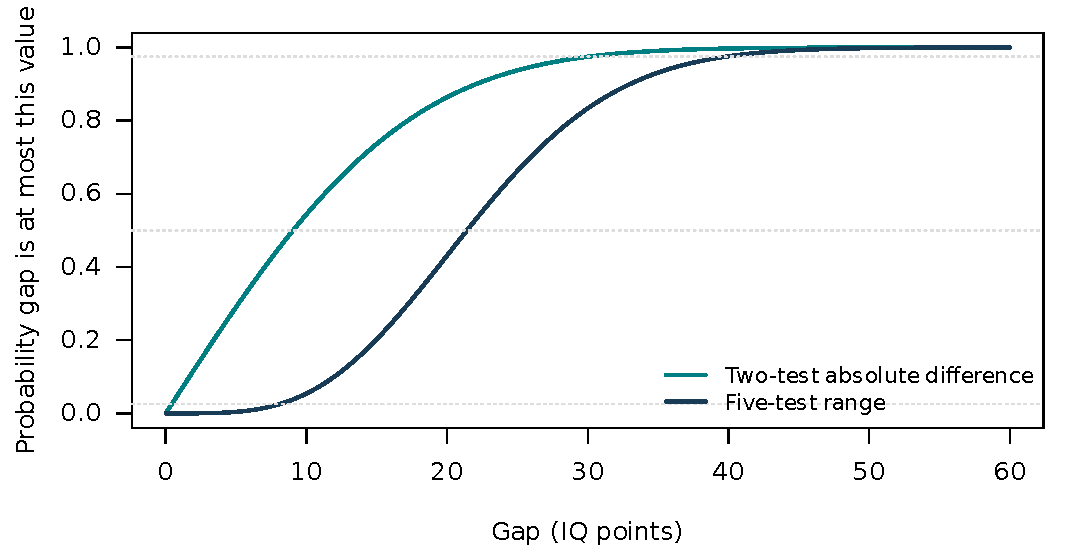
\includegraphics[width=.96\linewidth]{figures/distributions.pdf}
\caption{Model CDFs at SD 15 and correlation 0.6. Each curve gives the fraction
of people whose gap is at most the horizontal-axis value. Curves are theoretical,
not fitted to observations.}
\label{fig:distributions}
\end{figure}

\begin{table}[htbp]
\centering
\caption{Selected theoretical quantiles, in IQ points.}
\begin{tblr}{colspec={Q[c,wd=34mm] Q[r,wd=52mm] Q[r,wd=42mm]},
row{1}={font=\bfseries,bg=pale},hline{1,2,Z}={.5pt}}
Probability & Two-test absolute gap & Five-test range \\
0.025 & 0.420 & 8.061 \\
0.500 & 9.049 & 21.411 \\
0.950 & 26.296 & 36.597 \\
0.975 & 30.072 & 39.816 \\
\end{tblr}
\label{tab:quantiles}
\end{table}

The 2.5th and 97.5th percentiles delimit the central 95\% interval.
A threshold chosen to be exceeded by only 5\% of people instead uses the
95th percentile: 36.60 points for the five-test range. Neither interval is a
confidence interval for a true IQ or an estimated mean.

\begin{table}[htbp]
\centering
\caption{Percentage exceeding a specified gap under the main model.}
\begin{tblr}{colspec={Q[r,wd=40mm] Q[r,wd=45mm] Q[r,wd=45mm]},
row{1}={font=\bfseries,bg=pale},hline{1,2,Z}={.5pt}}
Threshold (points) & Absolute gap (\%) & Five-test range (\%) \\
5 & 70.94 & 99.59 \\
10 & 45.61 & 94.58 \\
15 & 26.36 & 79.71 \\
20 & 13.60 & 56.85 \\
30 & 2.53 & 16.64 \\
40 & 0.29 & 2.40 \\
\end{tblr}
\label{tab:tails}
\end{table}

The range exceeds 20 points for approximately 56.85\% of people, although one
specified pair differs by more than 20 points for only 13.60\%. There are ten
opportunities for a pairwise gap in a set of five, but they are dependent.
The range distribution accounts for that dependence exactly. Multiplying a
single-pair probability by ten, or treating all ten pairs as independent, would
not give the exact answer.

\section{A second-moment check}
\citet[section 1]{finch2016} also provides the iid five-normal range's second
raw moment, which in elementary inverse-trigonometric notation is
\begin{equation}
\nu_5=\E W_5^2=2\left[
1+\frac{5\sqrt3}{2\pi}
+\frac{15}{\pi^2}\arccos\frac23
-\frac{5\sqrt3}{2\pi^2}\arccos\frac14\right]
=6.15658306873\ldots.
\label{eq:range_second}
\end{equation}
Unlike the mean formula, this second-moment identity is imported from the
cited literature rather than proved here. Since $\E W_5=2a_5$,
\[
\operatorname{SD}(R_5)=s\sqrt{\nu_5-(2a_5)^2}=8.19740105668\ldots.
\]
The exact mean's Monte Carlo SE at five million independent people is
$8.19740105668/\sqrt{5{,}000{,}000}=0.0036659892$ points. This is a separate
check on the simulation's estimated SE of 0.0036653854.

\chapter{What the assumptions do: three counterexamples}
\label{ch:counter}

\section{Normal marginals and the complete correlation matrix are not enough}
A jointly normal law is much more restrictive than a list of normal marginal
distributions. \citet{dutta2014} construct non-Gaussian multivariate laws even
with all proper subvectors Gaussian. The simpler constructions below are proved
directly and are sufficient to refute identification from marginal normality
and correlations alone.

Let $B$ be Bernoulli with success probability $\rho$, independent of independent
standard normals $Z_0,Z_1,\ldots,Z_k$. Define
\begin{equation}
\widetilde X_j=
\begin{cases}
\mu+\sigma Z_0,&B=1,\\
\mu+\sigma Z_j,&B=0.
\end{cases}
\label{eq:mixture}
\end{equation}
Both conditional marginal laws are $N(\mu,\sigma^2)$, so the unconditional
marginal is exactly the same normal law. For $i\ne j$,
\[
\Cov(\widetilde X_i,\widetilde X_j)
=\rho\sigma^2+(1-\rho)0=\rho\sigma^2.
\]
Thus every pair has correlation $\rho$. When $B=1$, the range and absolute gap
are zero. When $B=0$, the scores are independent. It follows that
\begin{equation}
\E|\widetilde X_1-\widetilde X_2|=(1-\rho)\frac{2\sigma}{\sqrt\pi},\qquad
\E\widetilde R_k=(1-\rho)2\sigma a_k.
\label{eq:mixture_mean}
\end{equation}
At $\rho=0.6$ these expectations are 6.7702750 and 13.9555737 points.
The construction puts probability 0.6 on exactly identical scores. That makes
it an especially transparent proof, but is not intended as a realistic IQ model.

\section{A smooth counterexample without exact ties}
The failure of identification is not an artefact of that point mass.
Let a latent variable $C$ take the values $0.3$ and $0.9$ with equal probability,
and conditionally on $C=c$ let
\[
X_j=\mu+\sigma\sqrt c\,Z_0+\sigma\sqrt{1-c}\,Z_j.
\]
Each conditional marginal is $N(\mu,\sigma^2)$, irrespective of $c$, so every
unconditional marginal is normal. The covariance of any distinct pair is
$\sigma^2\E C=0.6\sigma^2$. Both component covariance matrices are positive
definite; the mixture has a smooth, positive density, and exact ties have
probability zero.

Conditional expectation gives
\begin{align*}
\E|X_1-X_2|&=\frac{2\sigma}{\sqrt\pi}\E\sqrt{1-C},\\
\E R_5&=2\sigma a_5\E\sqrt{1-C},
\end{align*}
where $\E\sqrt{1-C}=(\sqrt{0.7}+\sqrt{0.1})/2$.
This yields 9.7567093 and 20.1115132 points. Strict concavity of the square root
gives $\E\sqrt{1-C}<\sqrt{1-\E C}$ for nonconstant $C$, explaining why these
means are smaller than those of the single Gaussian model with the same
overall correlation. This comparison is specific to this mixture family; it
does not assert that the Gaussian law maximizes these expectations among all
possible laws with these moments.

\begin{table}[htbp]
\centering
\caption{Same normal marginals, same full correlation matrix, different answers.}
\begin{tblr}{colspec={X[l] Q[r,wd=35mm] Q[r,wd=35mm]},
row{1}={font=\bfseries,bg=pale},hline{1,2,Z}={.5pt},rowsep=3pt}
Joint law & Mean absolute gap & Mean range \\
Single Gaussian & 10.7047 & 22.0657 \\
Shared/independent mixture & 6.7703 & 13.9556 \\
Smooth Gaussian mixture & 9.7567 & 20.1115 \\
\end{tblr}
\end{table}

The main joint-normal assumption is sufficient, not logically necessary, for
the main numeric answers. Another law could happen to share them. What fails
is the claim that normal marginals and correlation force those answers.

\section{Even a Gaussian average correlation is not enough}
Let $(A,B)$ be jointly normal, with common mean $\mu$, SD $\sigma$, and
correlation $1/3$. Consider the five-vector
\[
\mathbf X=(A,A,A,B,B).
\]
There are four within-block pairs with correlation one and six between-block
pairs with correlation $1/3$. Their average correlation is
\[
\frac{4\cdot1+6\cdot(1/3)}{10}=0.6.
\]
Yet the five-test range is simply $|A-B|$, so
\[
\E R_5=2\sigma\sqrt{\frac{2/3}{\pi}}
=13.8197659789\ldots\text{ points at }\sigma=15.
\]
This is a singular Gaussian counterexample. It meets the weaker claim
``average correlation 0.6,'' not the stronger assumption that each pair has
correlation 0.6. Singularity is admissible for a probability counterexample;
the point is that an average discards information needed by a nonlinear
statistic such as the maximum-minus-minimum.

\section{Useful bounds from moments alone}
Without joint normality, Cauchy--Schwarz still gives
\begin{equation}
\E|D|\le\sqrt{\E D^2}=\sigma\sqrt{2(1-\rho)}.
\label{eq:boundabs}
\end{equation}
For equal means, variances, and equicorrelation, a range bound also follows.
Let $\bar X=k^{-1}\sum_jX_j$. For every realized vector,
\[
R_k^2\le2\{(\max_jX_j-\bar X)^2+(\min_jX_j-\bar X)^2\}
\le2\sum_j(X_j-\bar X)^2.
\]
The expectation of the last sum is
$k\sigma^2-k\Var(\bar X)=(k-1)\sigma^2(1-\rho)$. Therefore
\begin{equation}
\E R_k\le\sqrt{\E R_k^2}
\le\sigma\sqrt{2(k-1)(1-\rho)}.
\label{eq:boundrange}
\end{equation}
At the main parameters, these upper bounds are 13.4164 points for the absolute
gap and 26.8328 points for the five-test range. They are bounds under the moment
assumptions, not alternative Gaussian expectations. No claim of sharpness is
made for the specified normal-marginal class. General moment-based bounds for
order statistics are studied by \citet{bertsimas2006}; the elementary inequalities
above are derived here.

\chapter{Conditioning and sensitivity}
\label{ch:conditional}

\section{After a first score has been observed}
The question ``How far apart are two scores on average?'' differs from ``What
should I expect after obtaining a score of 145?'' The conditional normal formula
\citep{soch2020} gives, under the main bivariate model,
\begin{equation}
X_2\mid X_1=x\sim N\!\left(\mu+\rho(x-\mu),
                              \sigma^2(1-\rho^2)\right).
\label{eq:conditional}
\end{equation}
Thus $D\mid X_1=x$ has mean
$\delta_x=(1-\rho)(x-\mu)$ and SD $\tau_c=\sigma\sqrt{1-\rho^2}$.
Its expected absolute value is \cref{eq:folded} with those parameters.
Here $\tau_c=12$ points.

\begin{table}[htbp]
\centering
\caption{Conditional predictions at mean 100, SD 15, and correlation 0.6.}
\begin{tblr}{colspec={Q[r,wd=29mm] Q[r,wd=36mm] Q[r,wd=38mm] Q[r,wd=38mm]},
row{1}={font=\bfseries,bg=pale},hline{1,2,Z}={.5pt}}
First score & Mean second score & Mean signed gap & Mean absolute gap \\
85 & 91 & -6 & 10.747 \\
100 & 100 & 0 & 9.575 \\
115 & 109 & 6 & 10.747 \\
130 & 118 & 12 & 14.000 \\
145 & 127 & 18 & 18.703 \\
160 & 136 & 24 & 24.204 \\
\end{tblr}
\label{tab:conditional}
\end{table}

The conditional shift toward the population mean is regression to the mean
in this statistical model. It is not evidence of a causal decline in a person's
ability. The extreme-score rows also extrapolate the assumed normal model
into a region where real-test ceilings and calibration may matter.

\begin{figure}[htbp]
\centering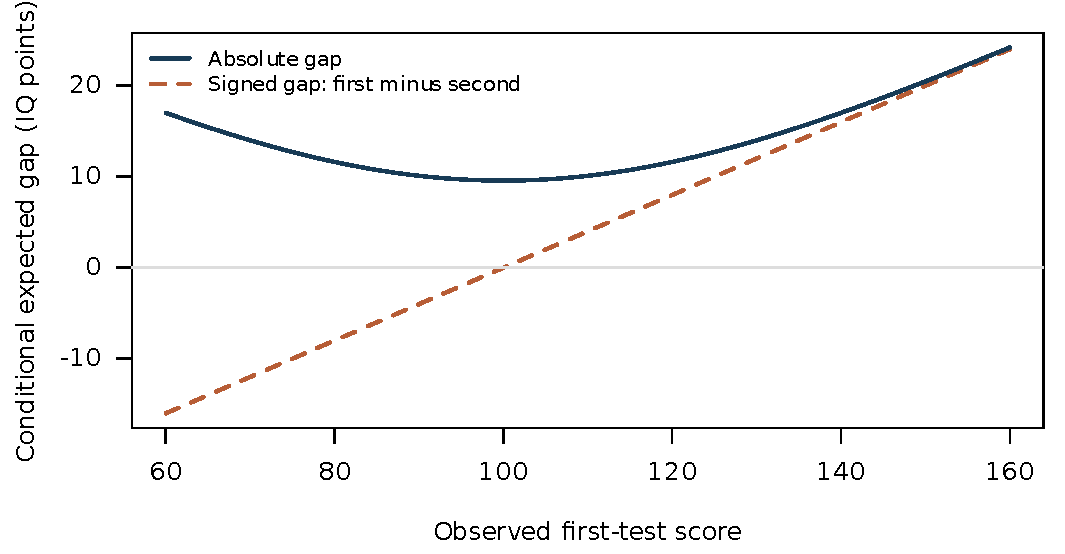
\includegraphics[width=.96\linewidth]{figures/conditional.pdf}
\caption{Conditional expected signed and absolute gaps after observing the first
score. The signed gap is first minus second. The model is symmetric about 100
for the absolute gap.}
\label{fig:conditional}
\end{figure}

For all remaining tests $j\ge2$, conditioning on $X_1=x$ gives means
$\mu+\rho(x-\mu)$, variances $\sigma^2(1-\rho^2)$, and off-diagonal covariances
$\sigma^2\rho(1-\rho)$. Their conditional correlations are $\rho/(1+\rho)$,
or 0.375 here. The first score is now fixed and the remaining four are still
dependent. Consequently the unconditional five-test range distribution cannot
simply be reused for a five-test range conditional on that first score.

\section{Selecting high scorers is different again}
Selecting everyone with $X_1>c$ is not equivalent to conditioning at $X_1=c$.
If $z=(c-\mu)/\sigma$, then the truncated-normal identity
$\int_z^\infty u\phi(u)\dd u=\phi(z)$ gives
\[
\E(X_1-X_2\mid X_1>c)
=(1-\rho)\sigma\frac{\phi(z)}{1-\Phi(z)}.
\]
This is another population average with a different inclusion rule. Membership
in a group selected on any of several scores, self-selection into testing, and
publication of only the best score create different conditioning events again.
The present report does not estimate those selection mechanisms.

\section{The range and the person's average score}
An instructive feature of the exchangeable Gaussian model is that $\bar X$ is
independent of the centered vector $(X_j-\bar X)_{j=1}^k$. Indeed,
$\Cov(\bar X,X_j-\bar X)=0$ for every $j$, and joint normality converts this
zero covariance into independence. Since the range is a function of that
centered vector, $R_k$ is independent of $\bar X$ under this exact model.
Conditioning on the \emph{average of all five} is therefore different from
conditioning on the \emph{first score}. This mathematical property should
not be presumed for real scores with unequal covariance structures.

\section{Changing the correlation, scale, or number of tests}
Both requested expectations scale linearly with $\sigma$ and, under the main
model, proportionally to $\sqrt{1-\rho}$.
For $f(\rho)=C\sqrt{1-\rho}$,
\[
f'(\rho)=-\frac{C}{2\sqrt{1-\rho}},\qquad
\frac{f'(\rho)}{f(\rho)}=-\frac1{2(1-\rho)}.
\]
Near 0.6, a correlation change of 0.05 corresponds to approximately a 6.25\%
oppositely directed change in either expectation. This is a local sensitivity,
not an uncertainty interval for a correlation estimate.

\begin{figure}[htbp]
\centering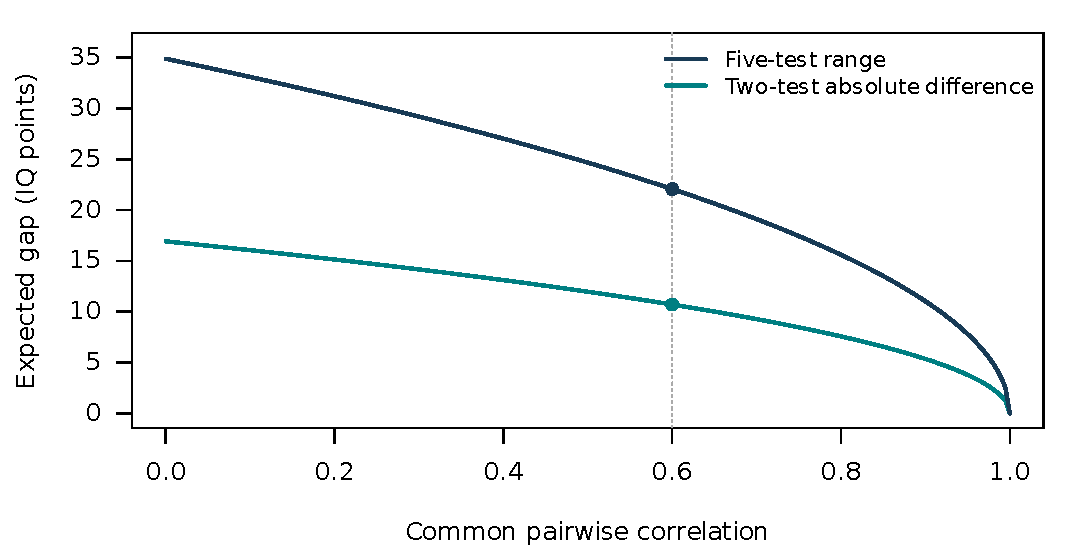
\includegraphics[width=.96\linewidth]{figures/correlation.pdf}
\caption{Correlation sensitivity at fixed SD 15. Both expectations shrink by
$\sqrt{1-\rho}$; the dots mark $\rho=0.6$.}
\label{fig:correlation}
\end{figure}

\begin{table}[htbp]
\centering
\caption{Sensitivity to the common pairwise correlation, with SD 15.}
\begin{tblr}{colspec={Q[r,wd=34mm] Q[r,wd=48mm] Q[r,wd=48mm]},
row{1}={font=\bfseries,bg=pale},hline{1,2,Z}={.5pt}}
Correlation & Mean absolute gap & Mean five-test range \\
0.0 & 16.926 & 34.889 \\
0.3 & 14.161 & 29.190 \\
0.5 & 11.968 & 24.670 \\
0.6 & 10.705 & 22.066 \\
0.7 & 9.271 & 19.109 \\
0.8 & 7.569 & 15.603 \\
0.9 & 5.352 & 11.033 \\
1.0 & 0.000 & 0.000 \\
\end{tblr}
\label{tab:sensitivity}
\end{table}

For a different common SD, multiply every point-valued answer by
$\sigma/15$. For example, SD 16 gives 11.4184 and 23.5367 points.
Adding more tests increases the range pointwise for nested test sets, whereas
the expected absolute gap for a specified pair stays unchanged.

\begin{table}[htbp]
\centering
\caption{Expected ranges for different numbers of equicorrelated tests, at SD 15 and $\rho=0.6$.}
\begin{tblr}{colspec={Q[r,wd=32mm] Q[r,wd=50mm] Q[r,wd=48mm]},
row{1}={font=\bfseries,bg=pale},hline{1,2,Z}={.5pt}}
Tests $k$ & $a_k=\E\max_jZ_j$ & Mean range (points) \\
2 & 0.564190 & 10.705 \\
3 & 0.846284 & 16.057 \\
4 & 1.029375 & 19.531 \\
5 & 1.162964 & 22.066 \\
10 & 1.538753 & 29.196 \\
20 & 1.867475 & 35.433 \\
50 & 2.249074 & 42.673 \\
\end{tblr}
\end{table}

\chapter{Psychometric interpretation and limits}
\label{ch:psychometrics}

\section{Intertest correlation is not automatically reliability}
The correlation in this report is the correlation between observed scores
across the specified population. Reliability concerns consistency over
specified replications of a measurement procedure. The
\citet{standards2014} distinguish internal consistency, alternate-form, and
test--retest approaches; Standard 2.4 specifically addresses precision of
interpreted score differences.

Under an additional parallel-test model $X_j=T+\varepsilon_j$, with one shared
true score, independent zero-mean errors, and equal error variances, the
intertest correlation can equal $\Var(T)/\Var(X_j)$. In that special model,
$\sigma\sqrt{1-\rho}$ is a standard error of measurement. Without those
assumptions, test-specific stable abilities, content differences, or other
nonshared influences can also contribute. The factor representation in
\cref{eq:factor} alone does not distinguish these possibilities.

For illustration, a Pearson technical report gives average reliability 0.95
for two particular WISC-V expanded indexes and 0.96 for FSIQ
\citep{raiford2015}. These publisher coefficients are neither correlations
between five distinct IQ tests nor substitutes for the stipulated 0.6.
Using a high internal reliability coefficient in an intertest discrepancy
formula without checking its interpretation can answer the wrong question.

\section{Agreement, discrepancy base rates, and population spread}
\citet{bland1986} explain why a high Pearson correlation need not indicate
close numerical agreement. Their analysis also highlights dependence on the
spread of the sampled population: correlations from a broad population need
not transfer unchanged to a restricted group.
The Gaussian difference distribution derived here is a population agreement
calculation under equal means and variances. It does not identify clinically
or educationally important discrepancies.

Pearson's score documentation distinguishes the statistical significance of
a discrepancy from its base rate in a normative sample
\citep{pearson2020,raiford2015}. The probabilities in \cref{tab:tails} are
\emph{model-based} base rates for an idealized set of tests; they are not
publisher-provided norms for a particular battery. In particular, a five-test
range of 30 points has probability approximately 16.64\% of being exceeded
under this model, so that gap alone is not exceptionally rare in the
modeled population.

Standard 2.20 in \citet{standards2014} addresses disclosure of adjustments for
range restriction. For this report, no adjustment can be calculated because
there is no actual sample or selection rule. The appropriate response is to
identify the population to which a correlation belongs before applying it.

\section{Practice and retest effects are real additional mechanisms}
Empirical studies show why occasion-specific means cannot always be assumed
equal. Three relevant examples were checked at abstract level:
\begin{itemize}
\item \citet{hausknecht2007} synthesized 50 studies with 107 samples and
134,436 participants in cognitive selection testing. Their adjusted overall
retest effect size was 0.26, with larger gains for coaching and identical forms.
The heterogeneous selection contexts do not justify a universal IQ-point correction.
\item \citet{estevis2012} studied 54 young adults, with mean age 20.9 and
initial mean FSIQ 111.6, retested on WAIS-IV after three or six months.
The abstract reports an approximately seven-point FSIQ gain.
The small, young, above-average sample and same-test design limit generalization.
\item \citet{scharfen2018} synthesized 174 samples from 122 studies, totaling
153,185 participants. The abstract reports retest effects moderated by test
content/operation, form equivalence, interval, and age, with no further
aggregate gains after the third administration in that synthesis.
That aggregate pattern is not a guarantee for a given individual or test.
\end{itemize}
These findings motivate more realistic models; they do not alter the
arithmetic of the hypothetical equal-mean Gaussian model. No detailed
moderator estimates or effect-size tables from unavailable full texts are used.

\section{Rounding, ceilings, and heterogeneous tests}
The normal model is unbounded. Actual reported scores may be discrete and
bounded; the WISC-V sample report explicitly documents bounded index and FSIQ
ranges \citep{pearson2020}. Such reporting rules can matter particularly near
the tails.

A simple deterministic rounding bound is available. If every score is rounded
to the nearest unit, each changes by at most 0.5 point. The absolute gap and
the range each change by at most one point, by the triangle inequality and
the fact that a maximum or minimum changes by at most the largest coordinate
perturbation. Thus their expectations change by at most one point under a
coupling to the same unrounded scores. This bound is conservative; it is not
an estimate of the actual rounding effect. The rounded scores' correlations
may also differ from the latent continuous correlations.

For known unequal means, variances, and a full covariance matrix $\Sigma$,
a multivariate-normal simulation can use a matrix factor $L$ satisfying
$LL^\mathsf T=\Sigma$ and generate $\symbf{\mu}+L\mathbf Z$.
The five-range simplification does not generally reduce to a single
$\sqrt{1-\rho}$ factor. Floor/ceiling rules, practice effects, or selection
should be represented explicitly if they are part of the intended estimand.

\chapter{Simulation design and actual results}
\label{ch:simulation}

\section{What the simulation is intended to establish}
The design specifies the aim, data-generating mechanisms, target expectations,
calculation methods, and checks. This follows the planning logic of the
ADEMP framework described by \citet{morris2019}. Here the experiment checks
known probability results, rather than comparing competing estimators on an
unknown empirical truth.

The main program uses base R only. It simulates 5,000,000 independent people
per model and five correlated scores per person, in batches of 100,000.
For each person it calculates one prespecified pair's signed, absolute, and
squared differences, plus the full range, maximum, and minimum. It also
accumulates all score means and covariances as a check on the data generator.

\texttt{rnorm} supplies the normal draws \citep{rnormal}.
The generator is explicitly set to Mersenne-Twister with inversion for normal
variates and rejection for sampling; the main seed is 20260903
\citep{rrng}. The shared/independent mixture continues the random stream
after the Gaussian run. Changing batch size changes draw ordering and can
change the realized sample, although not its target law. The seed alone is
not a complete specification of a run; script version, parameters, RNG kinds,
R version, and batch size also matter.

\section{Monte Carlo uncertainty}
If $T_i$ is one person's target statistic, then
\[
\widehat\theta=\frac1n\sum_{i=1}^nT_i,\qquad
\widehat{\operatorname{MCSE}}(\widehat\theta)
=\frac{s_T}{\sqrt n}.
\]
The code uses batch means and centered sums of squares, merging them using
the between-batch correction. This avoids subtracting two nearly equal large
raw second-moment accumulations. The approximate Monte Carlo interval is
$\widehat\theta\pm1.96\,\widehat{\operatorname{MCSE}}$.

The strong law applies because the person-level statistics are iid with finite
expectations. The central limit theorem applies to these sample means because
their variances are finite. In these normal and finite-normal-mixture models,
all the moments used exist. Thus Monte Carlo averages converge to the proved
model expectations. A finite run does not prove an identity or validate a model
for real IQ tests.

\begin{table}[htbp]
\centering
\caption{Fresh main R run: 5,000,000 people per model. Differences and ranges are in IQ points.}
\begin{tblr}{colspec={X[l] Q[r,wd=27mm] Q[r,wd=28mm] Q[r,wd=24mm] Q[r,wd=22mm]},
row{1}={font=\bfseries,bg=pale},hline{1,2,Z}={.5pt},rowsep=3pt}
Statistic & Theory & Simulated & MC SE & Error / SE \\
Gaussian signed gap & 0.000000 & 0.011731 & 0.005999 & 1.955 \\
Gaussian absolute gap & 10.704745 & 10.701215 & 0.003617 & -0.976 \\
Gaussian five-test range & 22.065699 & 22.063505 & 0.003665 & -0.599 \\
Mixture absolute gap & 6.770275 & 6.767670 & 0.005180 & -0.503 \\
Mixture five-test range & 13.955574 & 13.947077 & 0.008474 & -1.003 \\
\end{tblr}
\label{tab:simulation}
\end{table}

Both requested Gaussian expectations are within one estimated MC SE of
theory. The Gaussian mean signed gap is about 1.96 SE from zero, an ordinary
finite-sample fluctuation; its approximate 95\% Monte Carlo interval is
$[-0.0000269,0.0234885]$ points. It is not evidence of a systematic test bias.

The ten empirical Gaussian pair correlations range from 0.599650 to 0.600389.
Marginal test means range from approximately 99.99745 to 100.01079, and SDs
from 14.99656 to 15.00310. These are checks on a finite simulated sample,
not exact constraints imposed on that sample.

The newly executed main log is byte-for-byte identical to the earlier saved
log supplied by the preceding analysis. That verifies reproduction of the
reported run in this environment. It is not an independent random replication:
the seed and algorithm were intentionally held fixed.

\section{Separate smooth-mixture experiment}
The supplement runs 1,000,000 people, using seed 20260904, for the continuous
two-component model in \cref{ch:counter}.
\begin{center}
\begin{tblr}{colspec={X[l] Q[r,wd=31mm] Q[r,wd=31mm] Q[r,wd=29mm]},
row{1}={font=\bfseries,bg=pale},hline{1,2,Z}={.5pt},width=.92\linewidth}
Statistic & Theory & Simulated & MC SE \\
Absolute gap & 9.756709 & 9.760979 & 0.009218 \\
Five-test range & 20.111513 & 20.103200 & 0.012223 \\
\end{tblr}
\end{center}
Both deviations are below one MC SE. This is an actual run of the supplied
code, not a fabricated table of values chosen to match the formulas.

\section{Deterministic numerical checks}
\begin{enumerate}
\item Adaptive quadrature of \cref{eq:max_integral} agrees with the exact
five-normal formula to displayed precision; the reported integration error
estimate is about $4.21\times10^{-12}$. R's \texttt{integrate} uses adaptive
quadrature and supports infinite limits \citep{rintegrate}. Its error estimate
is numerical, not a formal mathematical enclosure.
\item The two-normal integral equals $1/\sqrt\pi$, checking that the general
range result reduces to the two-test absolute-gap formula.
\item The independently coded CDF integral agrees with \texttt{ptukey} at six
test arguments, with maximum observed absolute difference about
$4.28\times10^{-12}$. Inverting that integral independently confirms the
reported range quantiles; the 97.5th-percentile difference is about
$0.000003$ IQ point.
\item The factor-loadings covariance matches the target covariance matrix.
The supplement also checks the projection construction at correlations
$-0.25,-0.1,0,0.6,1$.
\item The exact second-moment calculation predicts the Gaussian range MC SE
independently of the simulated variance estimate.
\end{enumerate}
The simulation diagnostic flags deviations larger than six estimated SEs;
it is not a hypothesis test or a rule to keep changing seeds until a result
looks satisfactory. No such resampling was used to select the reported results.

\chapter{Evidence, conclusions, and unresolved questions}
\label{ch:evidence}

\section{Research approach and source quality}
Research was conducted on 3 September 2026 using targeted public web searches
and direct source reads. The search families were: normal order statistics and
five-normal range moments; Gaussian orthant probabilities; marginal versus
joint normality; equicorrelation matrices and moment bounds; correlation versus
agreement; psychometric reliability and discrepancy interpretation; cognitive
retest effects; and official R documentation for simulation and integration.

Examples of actual search targets included ``normal range expected maximum
five arcsin'', ``orthant probabilities Pinasco Smucler Zalduendo'',
``Bland Altman agreement correlation'', ``retest effects cognitive ability
meta-analysis'', and site-restricted searches for R's Tukey distribution and
random-number-generation documentation. This was a focused research synthesis,
not a registered systematic review or an exhaustive search of every database.

Primary papers, author-hosted manuscripts, official test-publisher documents,
the official testing standards, institutional documentation, and authored
probability proofs were prioritized. Research into mathematical foundations
and psychometric interpretation was divided between two additional AI research
workers; the coordinating assistant reconciled their findings, revisited key
sources, and checked the main calculations. These were not independent human
reviewers.

\section{What was verified, and at what level}
\begin{longtblr}[
caption={Evidence map and limits of access.},label={tab:evidence}
]{colspec={Q[l,wd=34mm] X[l] X[l]},rowhead=1,
row{1}={font=\bfseries,bg=pale},hline{1,2,Z}={.5pt},cells={valign=t},rowsep=3pt}
Claim family & Main evidence & Scope or limitation \\
Exact range mean & Finch; orthant identity in Pinasco et al.; proof in this report & Full relevant preprint passages checked. Formula is established, not a claimed new discovery. \\
Joint normality & Pishro-Nik; Taboga; Dutta and Genton & Full relevant sections checked; counterexamples in this report proved directly. \\
Covariance constraints & Archakov et al.; direct eigenvalue calculation & Relevant result read in a 2022 preliminary version; published metadata is from 2024. \\
Moment-only bounds & Bertsimas et al.; elementary bounds proved here & Full paper available. No claim that this report solves the sharp optimization problem. \\
Score scales and precision & Pearson sample/technical reports; 2014 Testing Standards & Relevant official sections read. Specific batteries do not validate the hypothetical five-test model. \\
Practice effects & Hausknecht et al.; Estevis et al.; Scharfen et al. & Original abstracts or author-associated abstract record only; full study methods and detailed tables not reviewed. \\
Simulation design & Morris et al.; official R manuals; actual R logs & Repository/abstract framework checked. Online R development docs and actual R 4.3.3 are distinguished. \\
Actual five-test applicability & None supplied & No named tests, real score matrix, or estimated target-population covariance. This remains unverified. \\
\end{longtblr}

The most consequential mathematical claim was checked through a self-contained
derivation, an independently tabulated literature formula, numerical integration,
and R simulation. The exact second-moment formula was taken from a cited source
and checked numerically, but not independently rederived. Searches stopped when
the substantive sections had adequate evidence and the remaining gap was lack
of real test data rather than lack of further general references.

\section{What a real-data extension would need}
To make an empirical prediction for particular tests, one would need their
identities and score scales, the target population and sampling/selection rule,
the full score matrix or a defensible covariance estimate, and administration
order, timing, prior exposure, and ceiling/floor information. Those data would
allow checks of mean/variance equality, covariance heterogeneity, discrepancy
distributions, tail behavior, and the effect of conditioning on an observed
score. If sampling uncertainty in the covariance were material, it would need
to be propagated into predictions, separately from Monte Carlo error.

\begin{resultbox}[title={\textbf{Supported conclusion}}]
For the explicitly assumed exchangeable joint-normal model, the requested
averages are rigorously established: \textbf{10.70 IQ points} for a two-test
absolute gap and \textbf{22.07 IQ points} for a five-test range.
Correlation 0.6 alone is insufficient, even with normal marginal score
distributions. The results are a mathematical benchmark whose empirical
applicability must be checked for the particular tests and population.
\end{resultbox}

\clearpage
\renewcommand{\bibname}{References}
\begingroup
\small
\bibliographystyle{plainnat}
\bibliography{references}
\endgroup

\appendix
\chapter{Reproducing the report}
\label{app:reproduce}

\section{Files and computational environment}
The source package contains the main XeLaTeX file, its complete body source,
the BibTeX database, two R programs, the workbook export program, build commands,
the actual run logs, vector figures, numeric CSV tables, and a companion
workbook. The simulations use only base R; the reported runs used R 4.3.3
(2024-02-29) on 64-bit Linux. Exact session details are in the logs.
The workbook is an export of model calculations and plotted values, not a
dataset of measured IQ scores.

The source-code appendices print every analysis, simulation, figure-generation,
workbook-export, and build program used in the deliverable. The XeLaTeX document
and bibliography sources are supplied as editable files in the package rather
than recursively printed inside their own output. External R, TeX, and workbook
library implementations are dependencies, not newly authored report code.

\section{Commands}
The complete build script below compiles the supplied sources and figures.
Its commented R commands can be run separately to reproduce the calculations:
\lstinputlisting[language=bash,numbers=none]{code/build_report.sh}
The first program refuses to overwrite an existing log. The supplement
regenerates its own derived tables, figures, and results. The precomputed vector
figures are included, so compiling the report alone does not require rerunning
the simulations or exporting the workbook.

The requested TeX components are loaded explicitly: \texttt{scrbook},
\texttt{fontspec}, \texttt{unicode-math}, \texttt{tcolorbox}, \texttt{tabularray},
\texttt{hyperref}, \texttt{bookmark}, \texttt{mathtools}, \texttt{microtype},
\texttt{scrlayer-scrpage}, and \texttt{cleveref}. Additional packages provide
geometry, figures, program listings, and author--year citations.
Duplicate package names in the request are loaded once; the intended hyperlink
package is spelled \texttt{hyperref}.

\section{Numeric data and precision}
The \texttt{tables} directory contains unrounded CSV values for the probability,
quantile, sensitivity, conditional, and counterexample tables, plus every
plotted curve. Calculations involving ordinary normal functions use R's double
precision. R documents \texttt{qtukey} accuracy at about the fourth decimal
place in its own units; the independent inversion check here agrees more
closely at the reported probabilities. Main-text range quantiles are therefore
rounded appropriately rather than presented as mathematically exact decimals.

The separate \texttt{iq\_report\_data.xlsx} workbook includes a formula-based
parameter sheet and the computed table/curve values, with units and source
notes. The exporter uses \texttt{@oai/artifact-tool}; it is optional for
reproducing the R results or the PDF. The complete export source is printed
for transparency, but users without that library can use the CSV files directly.

\chapter{Complete main R simulation source}
\label{app:maincode}
The following program is the unchanged simulation script from the preceding
analysis. It was executed again for this report. Its comments, input validation,
deterministic checks, accumulators, both model generators, output formatting,
and environment reporting are included in full.
\lstinputlisting[language=R]{code/iq_difference_simulation.R}

\chapter{Complete extension and export source}
\label{app:extensioncode}
\section{R calculations, smooth-mixture simulation, and figures}
\lstinputlisting[language=R]{code/iq_report_extensions.R}
\section{Companion workbook export}
\lstinputlisting[language=Java]{code/export_workbook.mjs}

\chapter{Complete AI-use disclosure}
\label{app:ai}

\begin{disclosurebox}[title={\textbf{Authorship and review status}}]
This report was generated with ChatGPT / Codex, provided by OpenAI, at the
request of Anders Hellström. AI assistance was substantive throughout the
research, mathematical presentation, programming, analysis, visualization,
and document production. It was not limited to proofreading or formatting.
No independent human mathematical or psychometric peer review is claimed.
\end{disclosurebox}

\section{Human contribution documented in the conversation}
The user posed the original questions about a two-test difference and a
five-test range at correlation 0.6, requested rigorous proof and an R
simulation, and subsequently requested an expanded, thoroughly sourced report.
The user specified XeLaTeX, KOMA-Script \texttt{scrbook}, narrow margins,
the principal packages, an unmissable opening AI disclosure, a complete closing
disclosure, and source-code appendices. The user did not supply an observed
IQ-score dataset or a set of named tests for empirical validation.
The numerical SD-15 and equal-mean conventions were modelling assumptions
made explicit in the preceding AI-assisted analysis and retained here.

\section{AI contribution}
The coordinating AI assistant recovered and read the preceding proof and R
script, assessed the assumptions, researched relevant public sources, and
developed the report's narrative and mathematical exposition. It verified the
two-test calculation, the cancellation argument for ranges, and the
five-normal closed form. It added explanations of the complete range
distribution, conditional prediction, sensitivity, bounds, a smooth-mixture
counterexample, an average-correlation counterexample, and the extension to
negative equicorrelation.

Two additional AI research workers performed bounded searches on mathematical
sources and psychometric interpretation. Their source records were reviewed
and integrated by the coordinating assistant. The workers used the same
general AI workflow and are not independent human validators. The exact
underlying model build identifier was not independently recorded for the
report; no unverified model-version label is asserted.

The AI wrote the supplementary R and workbook-export code, reran the original
R program, executed the supplementary computations, generated the vector
figures and numerical tables, and authored the XeLaTeX document and bibliography.
All newly authored computational programs are supplied in full.
The preceding main R script itself was also AI-generated, as disclosed in the
earlier conversation, and is preserved unchanged in this report package.

\section{Data, outputs, and checks actually performed}
No real participants were enrolled, and no observed IQ-test scores were
analysed. Every numeric data row used for simulation is pseudorandomly generated
under one of the stated models. The displayed simulation estimates are from
executed R code, with fixed seeds and saved session information. Literature
sample sizes and study findings are separately cited and were not merged into
the synthetic data.

The principal formulas were checked by analytic derivation, a published-source
comparison, quadrature, and Monte Carlo. The range CDF was evaluated by an
independent integral implementation as well as R's studentized-range functions.
The exact range second moment is explicitly attributed to Finch rather than
presented as independently proved. The repeated main run reproduced the
earlier log exactly. The supplementary smooth-mixture run used a different
fixed seed. Sources available only as abstracts and a result read in a
preliminary paper version are identified in the evidence chapter and references.

The PDF was compiled with XeLaTeX, checked for missing citations and layout
warnings, and visually reviewed on selected high-risk pages. This was sampled
visual inspection, not a claim that a human reviewed every page. Automated
structural checks and sampled visual checks do not establish mathematical or
empirical validity.

\section{Limits and responsibility}
AI systems can produce incorrect deductions, code, citations, or interpretations.
The checks documented above reduce particular risks but cannot exclude all
errors. Agreement among AI-generated derivations and simulations is especially
limited when both may share the same assumptions. The externally sourced exact
formula and the distinct numerical CDF implementation provide additional checks,
while applicability to actual IQ tests remains unverified.

The report is a mathematical and methodological analysis, not a personal IQ
assessment, a diagnosis, or evidence that particular real tests follow the
stated model. It claims no original discovery of the classical normal-range or
Gaussian orthant formulas. A reader intending to cite, publish, or apply the
report should evaluate its assumptions and calculations and retain the
substantive AI disclosure. Anders Hellström is identified as the requester;
the report does not attribute unobserved human review, endorsement, or
authorship of the AI-generated technical material to him.

\bigskip
\noindent\textbf{End of report.}
